% Use Deakin Title Page instead
% % Titlepage
% \title{ \huge{\textbf{\thesistitle{}}} \\[1.2cm]
% \large{Faculty of Science, Engineering and Built Environment\\
% Deakin University\\
% Melbourne, Australia\\}
% \vspace{1.2cm}
% \large{Submitted for the degree of Doctor of Philosophy} \\
% \vspace{1cm}
% }
% \author{ \Large{\textbf{\me{}}} }
% \date{\pubyear{}}
% \maketitle

%%% Abstract
% \newpage
%	\pdfbookmark[0]{Abstract}{abstract}

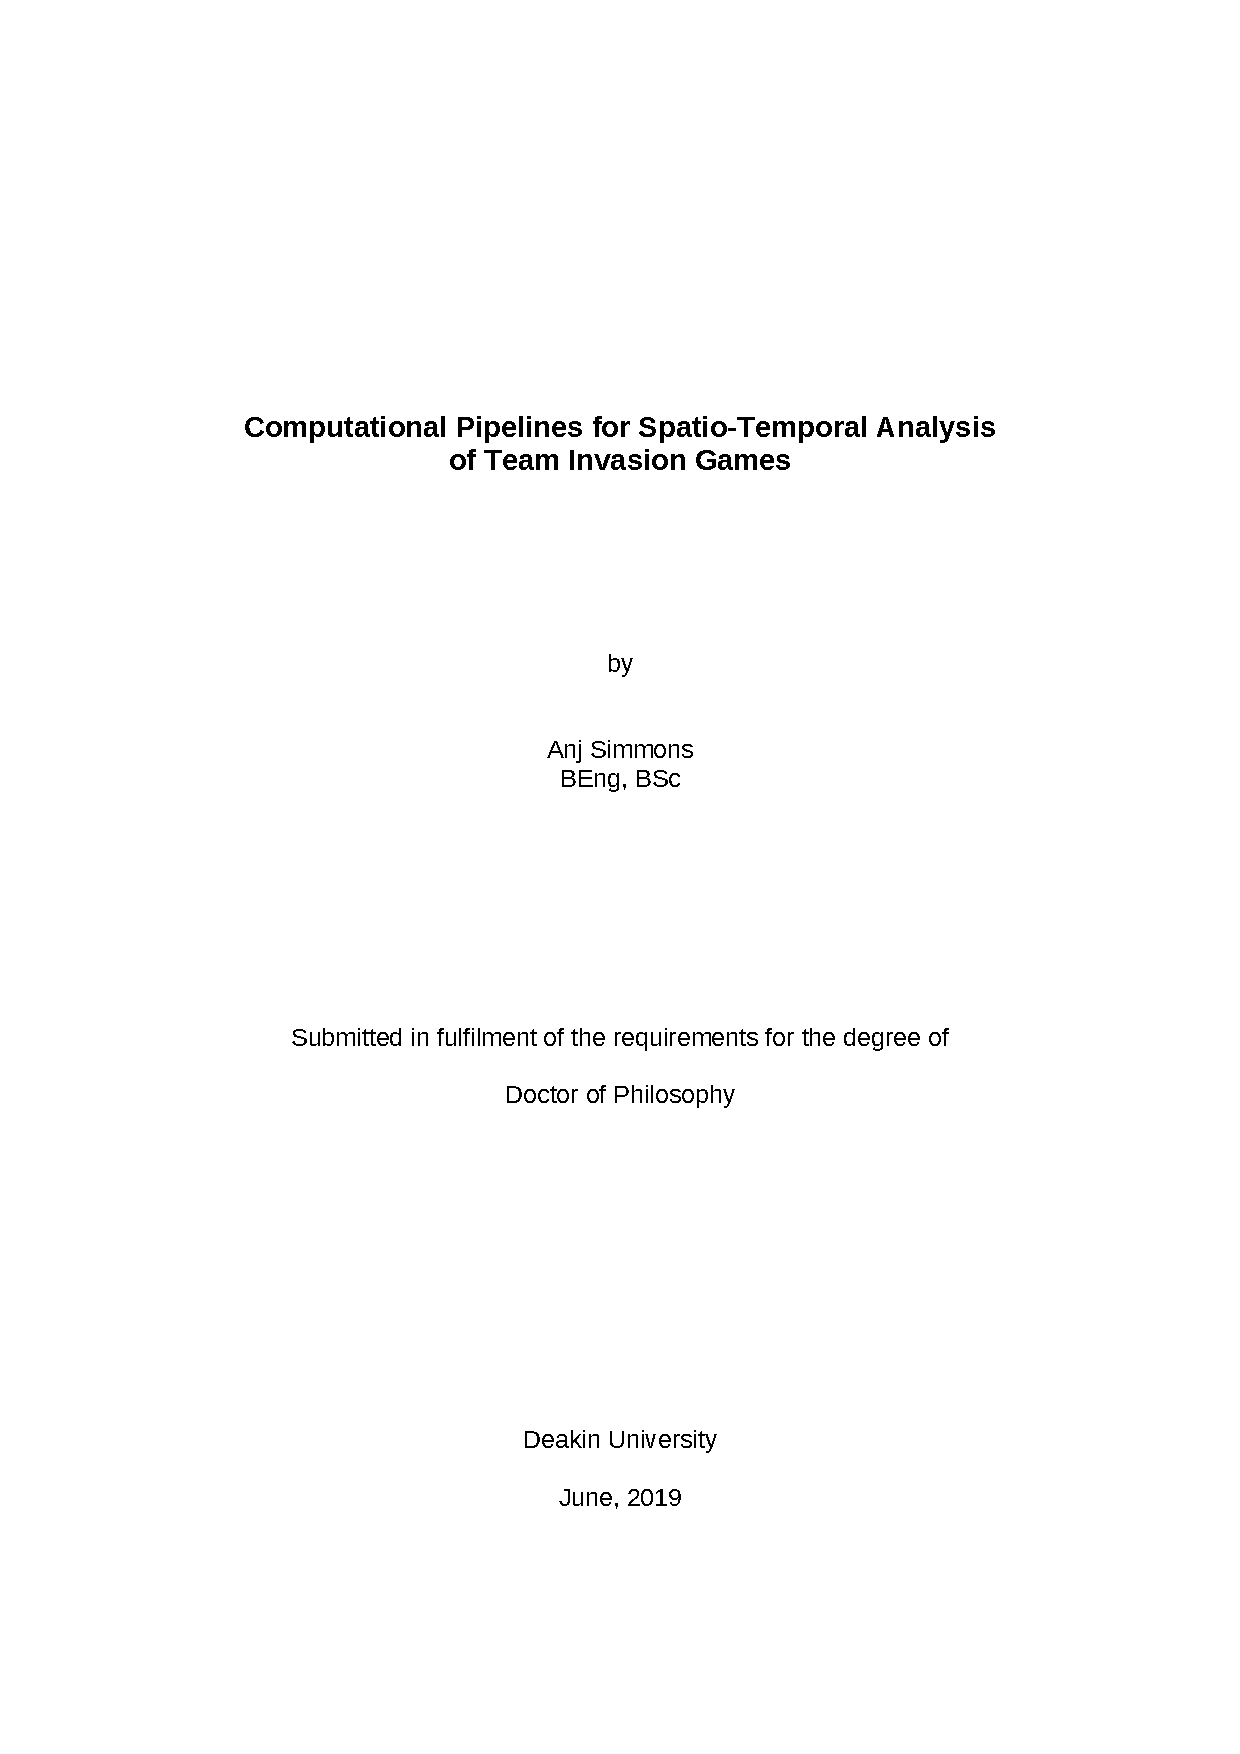
\includepdf{word/Sample-thesis-title-page-for-PhD-and-Masters-filled.pdf}
% Access to Thesis is just for library copy (add back later)
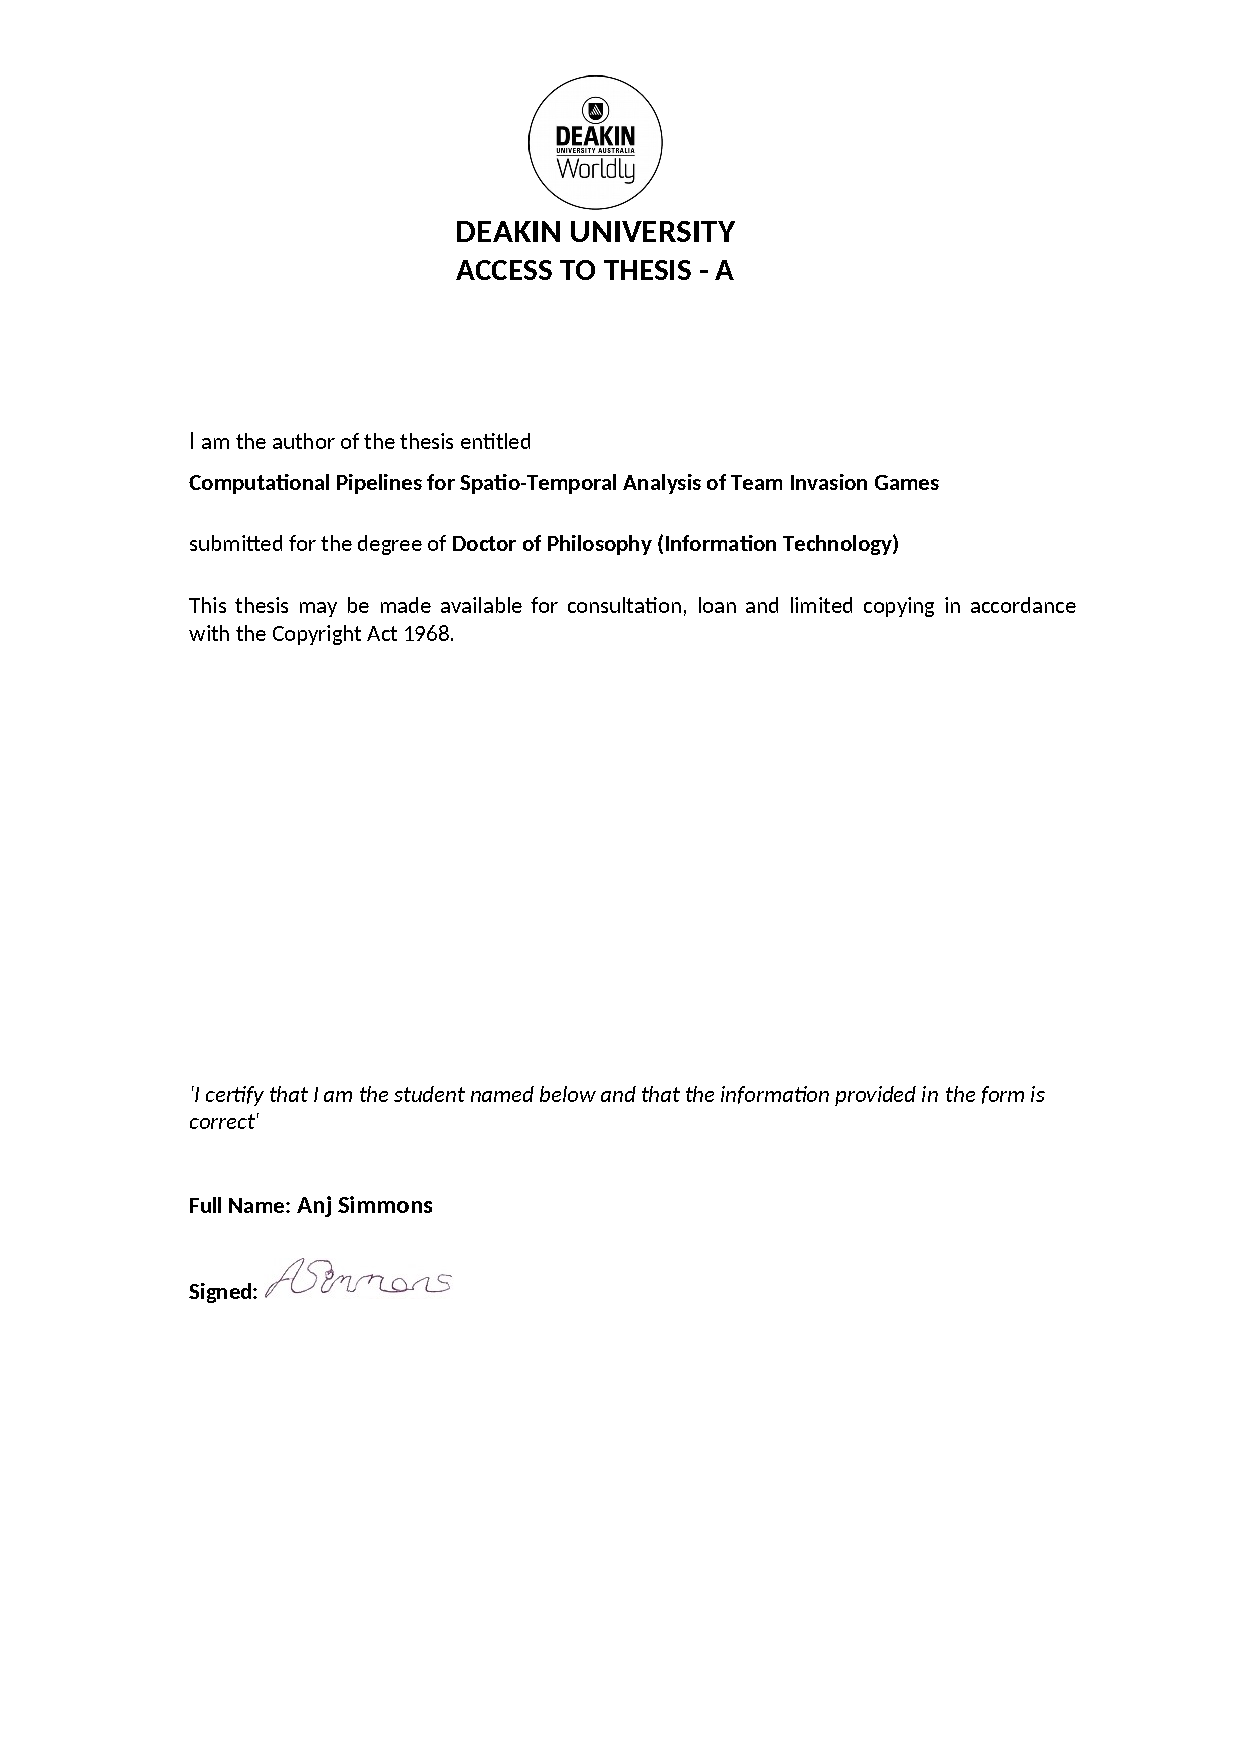
\includepdf{word/Access-to-thesis-form_v1-filled.pdf}

\includepdf{word/1-3-candidate-declaration-filled.pdf}

\chapter*{Abstract}
\vspace{-0.75cm}
\setstretch{1.12}
This thesis bridges the gap between raw position sensor measurements of individuals and high level strategic insights about group formations and behaviours. Specifically, it investigates the viability of GPS player tracking data in Australian Rules Football for strategy analysis and shows how characteristics of the sport domain affect the design of the data processing pipeline.

The core contribution of this thesis is a systematic investigation of the pipeline of transformation operations necessary to lift raw GPS player tracking data to a form that can be mined for insights relevant to a sport coach. For each component of the pipeline, the design decisions involved are identified and linked to the types of insights that can be extracted as well as the privacy implications for players. The methodology recognises the role of both manual and automated analysis processes in sport performance analysis as part of the processing pipeline. Data provenance standards are adapted to the context of sport to document the interplay of manual and automated analyses in a manner that is repeatable and auditable.

A review of common methods for data de-identification prevalent in the sport literature shows that: they are not suitable for position data; do not protect individual player privacy against data linkage attacks; and may be in violation of human ethics guidelines. This thesis addresses these shortfalls through a proposal to de-identify position tracking data by transforming them to a point~cloud representation (an unordered set of points) thus preventing re-identification of individuals while preserving the ability to perform spatio-temporal team-level analysis. To address the gap between theoretical techniques for privacy preservation and those used in practice, this thesis introduces a software tool and associated interaction model for data sharing that reduces the potential for human errors.

Given the unique nature of Australian Rules Football, there are special normalisation requirements to make effective use of positional data, as each field has a different shape and orientation. This thesis develops a novel technique for marking up coordinate systems at each venue to account for this.

Finally, a computational pipeline for Australian Rules Football is constructed using the techniques proposed in this thesis to demonstrate that they can be combined to provide meaningful team-level insights into formation changes during the game without compromising individual privacy.

% Skip Dedication
% Dedication
% \newpage \vspace*{8cm}
% \begin{center}
% 	\large Dedicated to all of my teachers, family and friends.
% \end{center}


% Acknowledgements
\chapter*{Acknowledgements}
\vspace{-0.5cm}
I would like to acknowledge with particular gratitude the assistance of my supervisors Prof. Rajesh Vasa, Prof. Paul Gastin, and Dr. Scott Barnett. I am also indebted to a number of other people, in particular, Prof. Kon Mouzakis, Dr. Clare MacMahon, Dr. Jacqueline Tran, and Daniel Hoffman who have contributed feedback and advice at various phases of the project.  I would also like to thank Hawthorn Football Club and Geelong Football Club for their assistance obtaining the datasets used in this thesis.

% I would also like to thank former analysts at %David Rath, Darren O'Shaughnessy,
%Hawthorn Football Club and the team at Geelong Football Club for their assistance obtaining and extracting sport player GPS data. % without which this project would not have been possible. %Pete Varszeghy, and Aaron Leis for their assistance obtaining and extracting sport player GPS data without which this project would not have been possible.

% \todo{Thank Clare, mathsport organisers (for teaching me what a conference could be - sport performance analysts with an interest in math, statistician interested in sport, coming together as a community (as opposed to ads and self-promotion))} % Clare thanked. No need to mention MathSport explicitly.

\vspace*{4cm}
\me{}, \pubyear{}

%	\pdfbookmark[0]{Acknowledgements}{acknowledgements}
% Declaration

% Use Deakin's declaration
% \chapter*{Declaration}
% \vspace{-0.5cm}
% %	\pdfbookmark[0]{Declaration}{declaration}
% I declare that this thesis contains no material that has been accepted for the award of any other degree or diploma and to the best of my knowledge contains no material previously published or written by another person except where due reference is made in the text of this thesis.
%
% \vspace*{4cm} \me{}, \pubyear{}
\chapter*{Publications Arising from this Thesis}
\vspace{-0.5cm}

% \nb{List of my pubs, not all of them are relevant to my thesis}

The work described in this thesis has been published as described in the following lists.

Publications highly relevant to this thesis:
\begin{enumerate}
  \item \fullcite{Simmons2017}
  \item \fullcite{Simmons2018}
  %\item \todo{Add Simmons et al 2018 "Emotional goals driven design of a data de-identification portal". OzCHI'18 (In Press)}
  % \item \todo{Add Simmons, Barnett, Vajda, Vasa 2018 "Data Provenance for Sport" (Work in progress)}
  \item \fullcite{simmons2018dataprov} \textit{(Draft)}
\end{enumerate}

\newpage

Other publications/presentations during candidature:
\begin{enumerate}
	\item \fullcite{Simmons2015}
  \item \fullcite{Simmons2016}
  \item \fullcite{Hoffman2018}
  % \item Daniel T. Hoffman, Andrew J. Simmons, Patrick Clifton, and Paul B. Gastin. ``The likelihood of winning decreases with one or more match injuries than the opposition in the Australian Football League''. \textit{(In Submission)}
  % \item Niroshinie Fernando, Mohamed Abdelrazek, Roopak Sinha, Andrew J. Simmons, Rajesh Vasa, Kon Mouzakis. ``Coping With Uncertainty: Building and Deploying Smart Home Apps''. \textit{(In Submission)} % IEEE Software rejected, finding new venue.
\end{enumerate}

\singlespacing

\tableofcontents
% Figure captions are too long and look terrible.
% \ifwip
%   \listoffigures \listoftables
% \fi
\newpage


%\chapter*{Commonly Used Acronyms}
%
%%	\pdfbookmark[0]{Commonly Used Acronyms}{acronyms}
%\begin{table}[h]
%	%\centering
%	\begin{tabular}{ll}
%%		Acronym&Full Form
%		\hline
%		RSN&Release Sequence Number\\
%%		\hline
%		OSS&Open Source Software\\
%		\hline
%	\end{tabular}
%\end{table}
